\section{The Jigsaw Puzzle Problem}
In the first part of this chapter we will discuss about the theory that has been using while setting the problem. In \ref{s:method} we will explain the implementation details that has been adopted to implement and improve the performance of the paper.\newline
An immediate approach to solve the Jigsaw puzzle is to stack the tiles of the puzzles along the axis of the color (so \(9\times3=27\) channels). However, with this approach the net is caused to learn only low-level texture similarities instead of high-level primitives. We as humans use kind of analogies between the tiles - like similar patterns or contiguous borders between pieces - as cues to solve jigsaw puzzles. However this learning does not require any understanding of the global object. Thus, we need a network that delays the computation of statistics across different tiles and that can find the parts arrangement using these features. The objective is to force the network to understand representative features that can discriminate the relative location of each part of an object.

% ------------------------------------------------------------------------------------------------ %

\subsection{The Context-Free Architecture}\label{ss:CFN}
The solution found in \cite{Noroozi_2016} is to build a siamese convolutional network (see fig. \ref{fig:siamese_network}), where AlexNet (until layer \textit{fc6}) is used for each crop of the puzzle, with shared weights. The outputs of all \textit{fc6} layers are concatenated and given as input to the fully connected layer \textit{fc7}. In this way each patch is given to a different AlexNet separately, until the very last fully connected layer: the \textit{fc7} is responsible for the understanding of the rearrangement of the tiles - the context of the objet. This is why this network architecture has been called \textit{context-free}: each patch remains separated from the others until the last layer that handles the context of the object. \newline
The performance of this architecture is similar to the AlexNet one in the classification task on the ImageNet 2012 dataset \cite{Imagenet_large_scale_hierarchical_image_database}. However the CFN is more compact than AlexNet: the first depends on \(27.5M\) parameters, the latter on \(61M\). In addition the network can be used interchangeably for different tasks including detection and classification.
\begin{figure}[!ht]
    \centering
    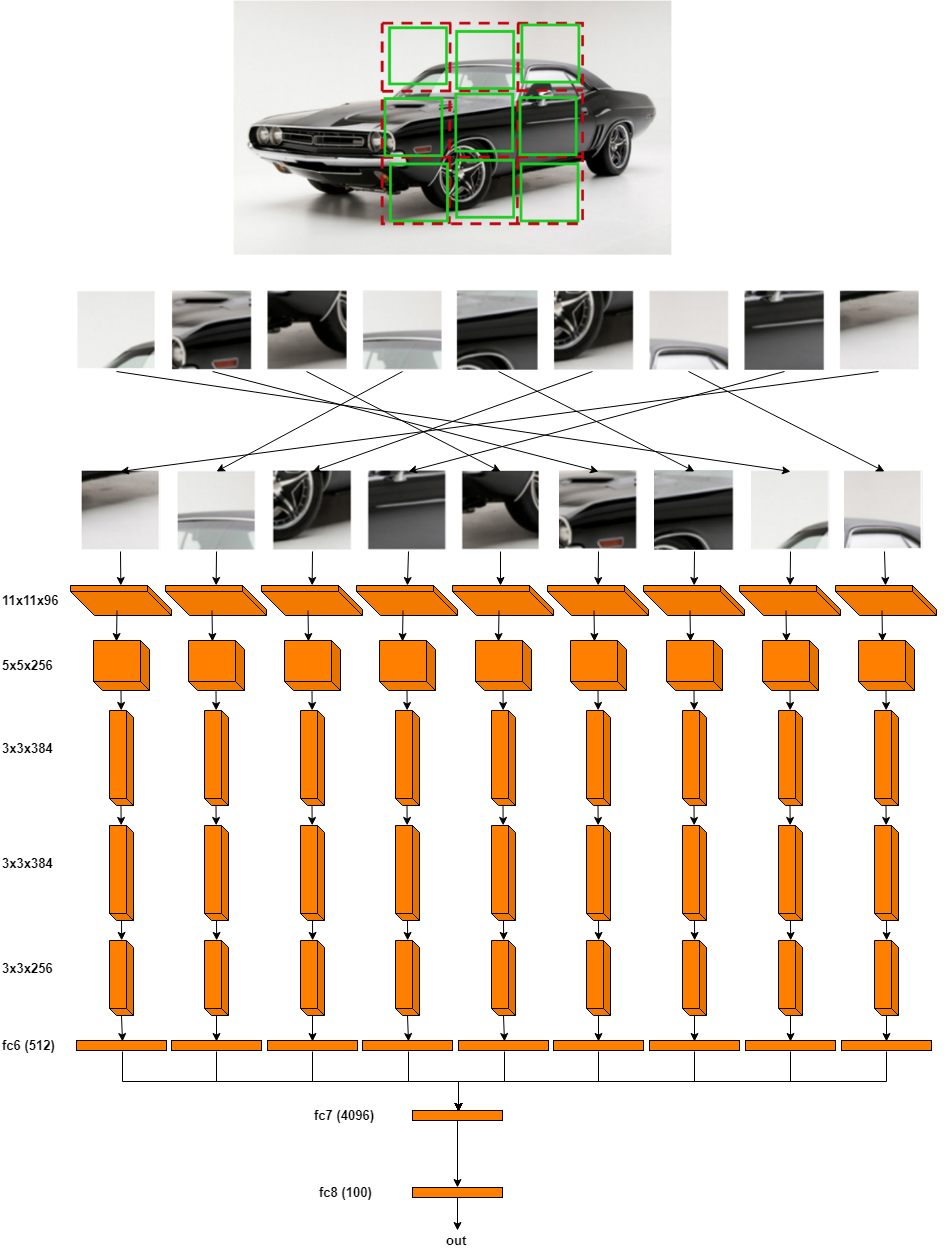
\includegraphics[scale=0.26]{images/Siamese_diagram.png}
    \caption{The Siamese network. The layers inside the AlexNet block have shared weights.}
    \label{fig:siamese_network}
\end{figure}
In the next section we show how to train the CFN for the Jigsaw Puzzle reassembly.


% ------------------------------------------------------------------------------------------------ %

\subsection{The Jigsaw Puzzle Task}
To train the CFN we define a set of Jigsaw puzzle permutation, \textit{e.g.}, a tile configuration \(S=(4, 2, 3, 5, 8, 7, 1, 0, 6)\). We randomly pick one of those permutations, rearrange the 9 input patches that has been retrieved from an image accordingly to that permutation, and ask the CFN to return a vector with the probability value for each index. Given \(9!=362,880\) possible permutations, it is clear that this is an important factor on the performance of the representation that the network learns. \newline
The permutation set controls the ambiguity of the task. If the permutations are too close to each other, the Jigsaw puzzle task is more challenging and ambiguous. For example, if the difference between two different permutations lies only in the position of two tiles and two of them are equal, the prediction of the right solution is impossible. To show this issue quantitatively, as specified in the ablation study of \cite{Noroozi_2016}[4.2], the learned representation on the PASCAL VOC 2007 detection task has been compared using several permutation sets based on the following two criteria:
\paragraph{Cardinality}
they trained the network with a different number of permutations to see what impact this had on the learned features. They found that as the total number of permutation increases, the training on the Jigsaw becomes more difficult. The performance of the detection task increases, though. As regard the experiments that we have made, we decided to use the first 100 permutations, as the paper results were promising and the training has shown to be easier than the 1000 task;
\paragraph{Average Hamming Distance}
it has been seen \cite{Noroozi_2016}[p.11] that the average Hamming distance between permutations controls the difficulty of the Jigsaw puzzle reassemlby task and is correlated with the object detection performance. As the average Hamming distance increases, the CFN gains higher accuracy and so does the fine-tuning tasks. For this reason we choose the higher possible Hamming distance. The algorithm that has been used is better described in Algorithm \ref{a:hm}: it begins with an empty permtation set and at each iteration it selects the one that has the maximum Hamming distance to the current permutation set.

\begin{algorithm}\label{a:hm}
    \caption{Generation of the \textit{maximal} Hamming distance permutation set}
    \SetKwInOut{Input}{Input}\SetKwInOut{Output}{Output}
    \SetKwData{P}{P}
    \SetKwFunction{repeat}{repeat}
    \SetKwFunction{until}{until}
    \SetKwFunction{hamming}{Hamming}
    \Input{N number of permutations}
    \Output{P maximal permutation set}
    \BlankLine
    \emph{// $\bar{P}$ is a $9 \times 9!$ matrix\;}
    $\bar{P} \leftarrow all \ permutations \ [\bar{P_1}, ..., \bar{P_9!}]$\;
    $P \leftarrow \emptyset$\;
    \emph{// uniform sample out of 9! permutations}\;
    $j \sim U[1, 9!]$\;
    $i \leftarrow 1 $\;
    \While{$i \leq{} N$}{
        \emph{// add permutation $\bar{P}_j $ to $P$}\;
        $P \leftarrow [P \ \bar{P_j}]$\;
        \emph{// remove $\bar{P}_j$ from $\bar{P}$}\;
        $\bar{P} \leftarrow [\bar{P}_1, ..., \bar{P}_{j-1}, \bar{P}_{j+1}, ...]$\;
        \emph{// D is a $i \times (9! - i)$ matrix)}\;
        $D \leftarrow \hamming{P, P'}$\;
        \emph{// $\bar{D}$ is a $1 \times (9! - i)$ row vector}\;
        $\bar{D} \leftarrow 1^T D$\;
        \emph{// $\bar{D}_k$ denotes the k-th entry of $\bar{D}$}\;
        $j \leftarrow \arg \max{}_k \bar{D}_k$\;
        $i \leftarrow i + 1$\;
    }
\end{algorithm}

% ------------------------------------------------------------------------------------------------ %

\subsection{Training the CFN}\label{s:training_CFN}
The output of the CFN can be seen as the conditional probability density function (pdf) of the spatial arrangement of object parts (or scene parts) in part-based model, \emph{i.e.},
\[p(S|A_1, ..., A_9)=p(S|F_1, ..., F_9)\prod_{i=1}^{9}p(F_i|A_i)\]
where $S$ is the configuration of the tiles, $A_i$ is the $i$-th part appearance of the object, and \{${F_i}$\}$_{i=1,...,9}$ form the intermediate feature representation. Our objective is to train the CFN so that the features $F_i$ have semantic attributes that can identify relative position between parts. As the pdf is very high-dimensional, close attention must be paid to the training strategy. In general, a self-supervised learning system might lead to representation that are suitable to solve the pre-text task, but not the target task, \emph{e.g.}, object classification, detection and segmentation. As regard this, an important factor to learn better representations is to prevent our model from taking undesiderable solutions, called solutions \textit{shortcuts}. In \cite{Noroozi_2016} they have used multiple techniques that apply to different problems:

\paragraph{Absolute position}
the CFN could learn to associate each appearance of $A_i$ to an absolute position. In this case, the feature $F_i$ carries no semantic meaning but just information about an arbitrary 2D position. To avoid this kind of learning we slowed down the training of the network in order to feed as much as possible Jigsaw puzzle per image; in addition the maximum Hamming distance and the randomic selection of those patch reassemblies assure us that different Jigsaw puzzle are choosen per each image with high probability. In this way the same tile should be assigned to multiple positions (ideally all 9) this making the mapping features $F_i$ to any absolute position equally likely.

\paragraph{Edge continuity}\label{p:edge_continuity}
to avoid shortcuts due to edge continuity and pixel intesity distribution we leave random gap between the tiles. In this way we discourage the network to learn context representation based on edges. During training the images are resized to a square of 256 pixels, preserving the original aspect ratio. Then they are cropped with a box of $225 \times 225$ randomly positioned and afterwards cropped into a $3 \times 3$ grid of $75 \times 75$ pixel tiles. From each of those tiles a $64 \times 64$ region is extracted randomly and then fed into the network. Thus, the average gap between each tile may range from a minimum of 0 pixels to a maxmimum of 22 pixels.

\paragraph{Chromatic aberration}\label{p:chromatic_aberration}
chromatic aberration is a relative spatial shift between color channels that increases from the image center to the borders. This type of distorsion helps the network to estimate the tile position. To avoid this kind of shortcut three techniques were applied:
\begin{itemize}
    \item crop central square of original image randomly, getting a $225 \times 225$ pixels image;
    \item at training time about the 30\% of the dataset is converted to grayscale
    \item spatial jitter over the color channels is applied randomly differently for each tile by $\pm0$, $\pm1$, $\pm2$ pixels. 
\end{itemize}
As shown in \cite{Noroozi_2016}[Tab.5], the application of all of these techniques makes the Jigsaw task more difficult - the accuracy is lower avoiding shortcuts - but the performance of the target task (detection in that case) is higher. So we decided to implement all of them.

% ------------------------------------------------------------------------------------------------ %

\textcolor{red}{"FOD DATASET: describe the data you are working with for your project. What type of data is it? Where did it come from? How much data are you working with? Did you have to do any preprocessing, filtering, or other special treatment to use this data in your project?"\newline
FOR METHOD: discuss your approach for solving the problems that you set up in the introduction. Why is your approach the right thing to do? Did you consider alternative approaches? It may be helpful to include figures, diagrams, or tables to describe your method or compare it with others.}

\subsection{The Dataset}
the dataset for the Jigsaw puzzle solver task is composed by squared images. Every images must be cropped into pieces, then fed into the Siamese network. No labels required. This is why we decided to use the Object Localization dataset \cite{ILSVRC15} of the ImageNet Large Scale Visual Recognition Challenge (ILSVRC2017). This dataset contains ~1.281M images for the training set, 50K validation images and 100K for the test. There are about 1K categories with a range from 732 to 1300 images each. All images are in JPEG format.

\subsubsection{Select and crop images}\label{sss:select_crop_image}
once the images has been downloaded we decided to build our own dataset on the basis of what we needed for the pre-task. So we prepared two datasets, both divided into 70\% training, 25\% validation and 5\% test:
\begin{itemize}
    \item one made of a total of 500K random images, that served the model trained with a personal computer;
    \item one made of a total of 1.4M random images, that served the model trained with a virtual machine hosted in Google Cloud Platform.
\end{itemize}
More information about the computational power is provided in section \ref{ss:machines}. For every image of both datasets we decided to:
\begin{itemize}
    \item select only RGB images;
    \item take the shortest dimension to crop the image to a squared proportion. The crop position was randomic;
    \item resize the cropped image to ($256 \times 256$) pixels with the Lancsoz algorithm;
    \item save the cropped resized image as new ones for further access.
\end{itemize}
Moreover we used the Welford's online algorithm \cite{Welford_online_algorithm} to calculate the mean and standard deviation of the training set, that was used later to make any scaled feature value the number of standard deviation away from the mean. This information, together with train, validation and test set dimensions has been stored inside a specific \emph{h5} file.

\subsubsection{The Hamming Set}
to create the Hamming set the algorithm \ref{a:hm} has been implemented. In particular we used the maximum euclidean distance between $P$ and $\bar{P}$. As regard the network on the personal computer, we decided to generate 40 permutations; for the GCP one 100 as this was the best compromise \cite{Noroozi_2016}[Tab.4] between the difficulty of the training of the pre-task and the results of the target task.

\subsubsection{The Data Pipeline}
for the implementation of the dataset we decided to use TensorFlow in Python. This was the best choice since we decided to use the same framework also for the design of the Siamese network (see \ref{ss:siamese}). We implemented the data stream trying to:
\begin{itemize}
    \item reduce the memory usage of the dataset both for RAM and GPU;
    \item speed up the data flow from the persistency to the GPU.
\end{itemize}
We decided to use the TensorFlow \emph{tf.data.Dataset} API \cite{tf_data_dataset}: this API provides many powerful tools to read images, manage the data stream and serve the dataset to the network.
In a first moment we decided to store the whole dataset inside a \emph{h5} format file, in which the images were store as \emph{numpy} arrays. In this way the dataset was a big blob file, easy to manage and access. With this kind of persistency, we created a generator that read the images one at a time and serve to the \emph{Dataset from generator} API of TensorFlow. This approach was succesfull because there was a minimum memory usage since every image was loaded in a binary mode. While in the personal computer all the resources were used, once we moved to the Google Cloud Platform we realized that the online GPU was barely exploited. This was because the GPU was much powerful and it processed much more images than the generator could provide. 
So we decided to change approach: first we saved the images produced in \ref{sss:select_crop_image} as new images on disk. Then we collected the all paths to the images, and let the \emph{tf.io} API to read them. In this way the shuffling was applied to very little string object, and the TensorFlow API was responsible for reading and parsing every image in a concurrent way.\newline
As regard the data transformations, we implemented every step in \ref{s:training_CFN}. We implemented every transformation as a \emph{lambda} python callable function, that we included in the \emph{tf.data.Dataset} pipeline with the specific \emph{dataset.map} method. This let TensorFlow to manage the reading and preprocessing of the images within the computational graph, in a concurrent (and distributed, if necessary) manner, mainly with the GPU cores. The steps are the following:
\begin{enumerate}
    \item we created the list of paths to train/val/test images and a random list of permutation indexes of the same lenght of the list of paths; in addition, a pointer to the \emph{h5} information file described above. This file is useful to determine the dimension of the sets together with the mean and standard deviation of the training set at compile time, sparing computational power. The list of permutation indexes is generated every repetition of the dataset randomly, so the labels are always different for each epoch;
    \item we provided the two lists to TensorFlow \emph{tf.io} API, which is responsible for taking one element at a time. It also gives an "imperative" way-of-programming to implement the data pipeline;
    \item now the image is a tensor of float array of numbers. From every image is subtract the training mean and it is divided for the training variance as specified in \ref{sss:select_crop_image};
    \item with a probability of 30\% the image is then converted to grayscale within the training set;
    \item the image is cropped as described in the section \ref{p:edge_continuity}: every operation (multiplication, addition, slicing, ecc) is made with the TensorFlow methods and types to keep the computation efficient;
    \item every crop is jittered spatially as described in \ref{p:chromatic_aberration};
    \item the label is converted in the OneHot format;
    \item the dataset is now served.
\end{enumerate}

\subsection{The Siamese Neural Network}\label{ss:siamese}
The architecture of the Siamese Neural Network, within the AlexNet one, has been well defined in \ref{ss:CFN} and in \cite{alexnet_paper}. Although the number of layers and the dimension of the kernels were strictly defined, we was quite free on the definition of the optimizers, the regularizers and the parameters. In addition, we also tried to insert some other layers - mainly batch normalization ones -, since it has been demonstrated \cite{batch_norm_paper} that the reduction of the covariate shift between internal layers can speed up training. In the next sections we will discuss about the framework that we used and the two planned networks

\subsubsection{TensorFlow and the \emph{eager execution}}
TensorFlow's eager execution \cite{tf_eager} is an imperative programming environment that evaluates operations immediately, without building grapgs: operations return concrete values instead of constructing a computational graph to run later. This makes it easy to get started with TensorFlow and debug models, and it reduces boilerplate as well. Eager execution is a flexible machine learning platform for research and experimentation and provides:
\begin{itemize}
    \item \textit{an intuitive interface}: the programmer can structure the code naturally and use Python data structures;
    \item \textit{easier debugging}: the operations can be called directly and be inspected by standard Python debugging tools;
    \item \textit{natural control flow}: it can be used the Python control flow instead of the graph one, simplifying the specification of dynamic models.
\end{itemize}
We made the first implementation of the Jigsaw puzzle solver method with the computational graph. The debugging was painful; in addition, since the architecture is not a standard one, we encountered many troubles with the operations to be attached to the computational graph, such as the loss and accuracy ops. This is why we decided to move to this new framework and to implement the Jigsaw puzzle solver network from scracth.\newline
Since we needed a Siamese network with shared weights, we could not take benefits from the \emph{models} that \emph{tf.keras} offers. So we implemented the pre-task neural network as a subclass of the \emph{tf.keras.Model} API. This \emph{Model} class exposes built-in training, evaluation and prediction loops; in addition, it gives the list of its inner layers and the saving and serialization APIs. In this way we wrote all the layers that we needed in the initialization of the class (the AlexNet's layers and the following ones). Then we set the behaviour of the \emph{call} function so:
\begin{enumerate}
    \item the \emph{AlexNet} block is called many times as the number of crops: the inputs are the different tiles, one per AlexNet;
    \item the outputs (the \textit{fc6} layers, one per each AlexNet of the block) are collected and concatenated;
    \item the concatenation is then provided to the dense and then the output layer is computed.
\end{enumerate}
This configuration let us save and restore the weights easily for the target task, since the architecture remains mostly the same, apart from the \emph{call} method.

\subsubsection{The PC architecture}
We calls the architecture that we trained in the personal computer the "PC" architecture, in contrast with the "GCP" one that we trained in Google Cloud Platform.\newline
The PC network is well represented in fig. \ref{fig:PC_net}.
\begin{figure}[!ht]
    \centering
    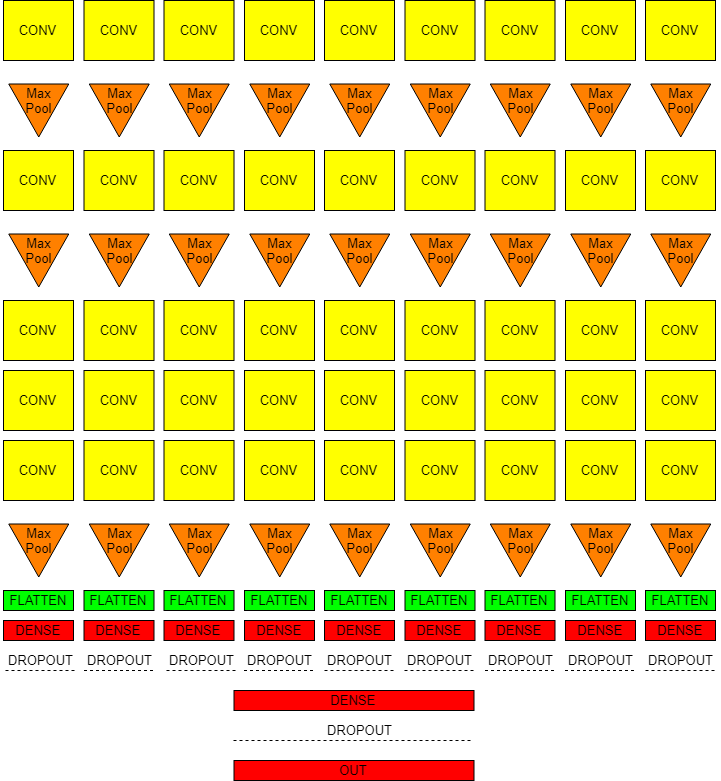
\includegraphics[scale=0.26]{images/PC_net.png}
    \caption{Architecture of the PC neural network.}
    \label{fig:PC_net}
\end{figure}
In this architecture we implemented all the features that were present in the original paper \cite{Noroozi_2016} with no addictions. All the activations are \emph{relu}s, the dimensions of the kernels are already listed in fig. \ref{fig:siamese_network}. We used the Stochastic Gradient Descent optimizer as precised in the previous article. More information about the parameters and the training tactics are presented in \textcolor{red}{REFER TO SECTION EXPERIMENTS}

\subsubsection{The GCP architecture}

\subsection{Machine details}\label{ss:machines}